\documentclass[12pt]{article}
\usepackage{alltt}
\usepackage[utf8]{inputenc}
\usepackage[dvips]{graphicx}
%\usepackage{a4wide}
\usepackage{epsfig}
\usepackage{fancybox}
\usepackage{verbatim}
\usepackage{array}
\usepackage{latexsym}
\usepackage{alltt}
%\usepackage{dsfont}
\usepackage{caption}
\usepackage{subcaption}
%\usepackage{fullpage}
\usepackage{hyperref}
\usepackage{textcomp}
\usepackage{listings}
\usepackage{color}
\usepackage{amsmath}
\usepackage{amsfonts}
\usepackage{tikz}
\usepackage{float}
\usepackage{matlab-prettifier}
\usepackage{graphicx}

\usepackage[hmargin=3cm,vmargin=6.0cm]{geometry}
%\topmargin=0cm
\topmargin=-2cm
\addtolength{\textheight}{6.5cm}
\addtolength{\textwidth}{2.0cm}
%\setlength{\leftmargin}{-5cm}
\setlength{\oddsidemargin}{0.0cm}
\setlength{\evensidemargin}{0.0cm}

%misc libraries goes here

\begin{document}

\section*{Student Information } 
%Write your full name and id number between the colon and newline
%Put one empty space character after colon and before newline
Full Name : Doruk Berke Yurtsizoglu \\
Id Number :  2522225\\

% Write your answers below the section tags
\section*{Answer 1}

\subsection*{a)} 

Sum of the 16 different measurement results is: 108.9\\
Sample mean of these measurement results, $\mu$, is: 108.9/16 = 6.8\\
Count, N: 16\\
$\alpha$: 1 - 0.98 = 0.02\\
\\
$\sigma^2$ = $\dfrac{\sum (x_i - \mu)^2}{N-1}$ = 16.70/15 = 1.113\\
\\
$\sigma$ = 1.05\\
Margin of Error = $Z_{\alpha /2}$ * $\dfrac{\sigma}{\sqrt{N}}$ = 2.60 * 1.05/4 = 2.60 * 0.25 = 0.68\\
Confidence Interval = 6.8 $\pm$ 0.65 = $[6.12, 7.48]$\\


\subsection*{b)} 

$\alpha$: 0.05\\
t-value for $\alpha$ = 0.05, df = 15: 1.753\\
\\
$\dfrac{6.8 - 7.5}{(1.05)/\sqrt{16}}$ = -2.62 which is not in the interval $-1.753 < t < 1.753$. So, it is in the rejection zone. We can say that the improvement is effective. (Reject Null,  Null Hypothesis = Improvement is not effective)\\

\subsection*{c)} 
We can reach to a conclusion without doing any calculation. If the car is consuming 6.5 litres instead of 7.5 litres; since the sample mean is 6.8 which is greater than 6.5, we can conclude that the $t$ value is not in the rejection zone. We are able to conclude like that because both $\sigma$ and $\sqrt{N}$ are positive.



\section*{Answer 2}

\subsection*{a)}
$H_0$ = 5000\\
$H_A$ $>$ 5000\\
\\
The claim of Ali is the null hypothesis. 

\subsection*{b)} 
$\alpha$: 0.05\\
t-value for $\alpha$ = 0.05, df = 99 is approximately 1.66\\
\\
$\dfrac{5500 - 5000}{(2000)/\sqrt{100}}$ = 2.5 which is greater than 1.66. So, it is in the rejection zone. Since our value is in the rejecting zone, Ahmet can claim there is an increase in the rent prices. (Reject Null)\\

\subsection*{c)} 

We can calculate the p-value by using the z-score of 2.5 from the table.\\
p-value = $1 - \Phi (2.5)$ = 1 - 0.9938 = 0.0062\\
Since p-value is smaller than 0.01, we can reject the null hypothesis.\\


\subsection*{d)} 
Sample mean, $\mu$: $Mean_{istanbul} - Mean_{ankara}$ = 6500 - 5500 = 1000\\
$\sigma$(ankara): 2000 \\
$\sigma$(istanbul): 3000 \\
$\sigma$(sample mean): $\sqrt{\dfrac{2000^2}{100} + \dfrac{3000^2}{60}}$\\
\\
$\alpha$: 0.01\\
$Z_a$ = 2.326\\ 
\\
$Z_a > \dfrac{6500 - 5500}{\sqrt{\dfrac{2000^2}{100} + \dfrac{3000^2}{60}}} =  \dfrac{1000}{\sqrt{\dfrac{2000^2}{100} + \dfrac{3000^2}{60}}}$ = 2.294
\\ 
\\
Since $-Z_a < t < Z_a$, it is in the non-rejecting zone.\\
\section*{Answer 3}
Let's say:\\
$H_0$: Independent\\
$H_A$: Dependent\\
\\
chi-square = $\sum (observed - expected)^2 / expected$\\
expected = (row total * column total) / total\\
\\
For winter:\\
Expected rain: $\dfrac{(34+56)*(34+32+15+19)}{34+32+15+19+56+58+75+71}$ = 25\\
\\
Expected non-rain: $\dfrac{(34+56)*(56+58+75+71)}{34+32+15+19+56+58+75+71}$ = 65\\  
\\
Since rainy and non-rainy days of each season is equal to each other, there is no need to calculate the other seasons expected values. They all will have 25 expected rainy days and 65 non-rainy days.\\
Now we have all the information to calculate the chi-square value. Let's start:\\
\\
chi-square: $((34-25)^2 / 25 + (56-65)^2 / 65) + ((32-25)^2 / 25 + (58-65)^2 / 65) + ((15-25)^2 / 25 + (75-65)^2 / 65) + ((19-25)^2 / 25 + (71-65)^2 / 65)$
\\
chi-square: 14.73\\
degree of freedom: (2-1)*(4-1) = 3\\
\\
From the chi-square table, it cn be observed that the p-value is between 0.005 and 0.001. If we choose level of significance as $\% 5$, then the result is significant which states that we need to reject the null hypothesis. So, the rainy days are dependent to seasons.\\ 
\section*{Answer 4}

\subsection*{a)} 

\begin{lstlisting}[style=Matlab-editor]

% Observed frequencies
observed = [34 56; 32 58; 15 75; 19 71];

% Calculate row totals, column totals, and total sum
row_totals = sum(observed, 2);
col_totals = sum(observed, 1);
total_sum = sum(row_totals);

% Calculate expected frequencies assuming independence
expected = row_totals * col_totals / total_sum;

% Calculate chi-square value
chi2_value = sum((observed(:) - expected(:)).^2 ./ expected(:));

% Degrees of freedom
df = (size(observed, 1) - 1) * (size(observed, 2) - 1);

% Calculate p-value
p_value = 1 - chi2cdf(chi2_value, df);

% Display chi-square value and p-value
fprintf('Chi-square value: %.2f\n', chi2_value);
fprintf('P-value: %.7f\n', p_value);

\end{lstlisting}

\begin{figure}[H]
  \centering
  \begin{subfigure}[b]{0.4\linewidth}
    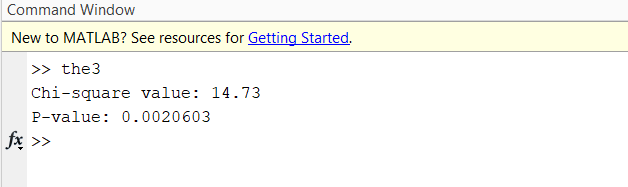
\includegraphics[width=\linewidth]{Screenshot (1885).png}
    \caption*{Printed Result of the Code Above}
  \end{subfigure}
\end{figure}



\end{document}